\documentclass{beamer}
\usepackage[utf8]{inputenc}
\usetheme{Madrid} % Adds bottom bar and title box
\usecolortheme{default}

\title{\subtitle{Binary Classification Model for Decay Events}}
\author{Prince Bhaura, Yijie Wang, Murdock Aubry}
\institute{University of Toronto}
\date{\today}


% To compile: 
% 				pdflatex slides
% To clean: 
% 				rm -f *.aux *.log *.nav *.out *.pdf *.snm *.toc

% Overall structure:
% 
% 	1. Discuss pre-existing model
% 		a) Pros and cons
% 		b) Characterize requirements of input data
% 		c) Discuss simplifications that can be made to implement 
% 				binary classification and possiblilities of a speedup
% 
% 	2. Discuss specific data sets that will be provided to our model
% 		a) What is different from data used in other model 
% 		b) key pieces of information
% 
% 	3. Outline the proposal for the new model
% 		a) Specifics about implementation, architecture, optimization methods...


\AtBeginSection[]
{
  \begin{frame}
    \frametitle{Table of Contents}
    \tableofcontents[currentsection]
  \end{frame}
}

\begin{document}

\frame{\titlepage}

\begin{frame}
	\frametitle{Table of Contents}
	\tableofcontents
\end{frame}





\section{NuGraph GNN}

\begin{frame}
	\frametitle{Introduction to NuGraph}
	% Simple and coherent introduction to the class of model we are working with and its primary operations
		\begin{enumerate} 
			\item NuGraph is a graph neural network (GNN) designed for reconstructing particle interactions in neutrino physics detector environments.

			\item Trained and tested on DUNE data, this model is primarily used for the classification of detector hit particle type.

   			\item Secondary functions include background hit rejection, event classification, clustering and vertex reconstruction.
		\end{enumerate}

		\centering
		\vspace{\fill}
		Github: \href{https://github.com/exatrkx/NuGraph/tree/main}{\color{blue} NuGraph}
\end{frame}

\begin{frame}
	\frametitle{Three Flavour Paradigm}
	% I think it is important that we provide sufficient motivation for designing this model
	% Here we should describe the three flavour paradigm, motivations for classifying particle flavour
\end{frame}


\begin{frame}
	\frametitle{Data Collection: Time Projection Chamber}
	% Discuss specific data collection methods 
	% both SP and DP, but mainly focus on the overall ideology and methods for doing so
	% Why is the information collected from the LArTPC sufficient for classification purposes?
	\begin{figure}[h!]
		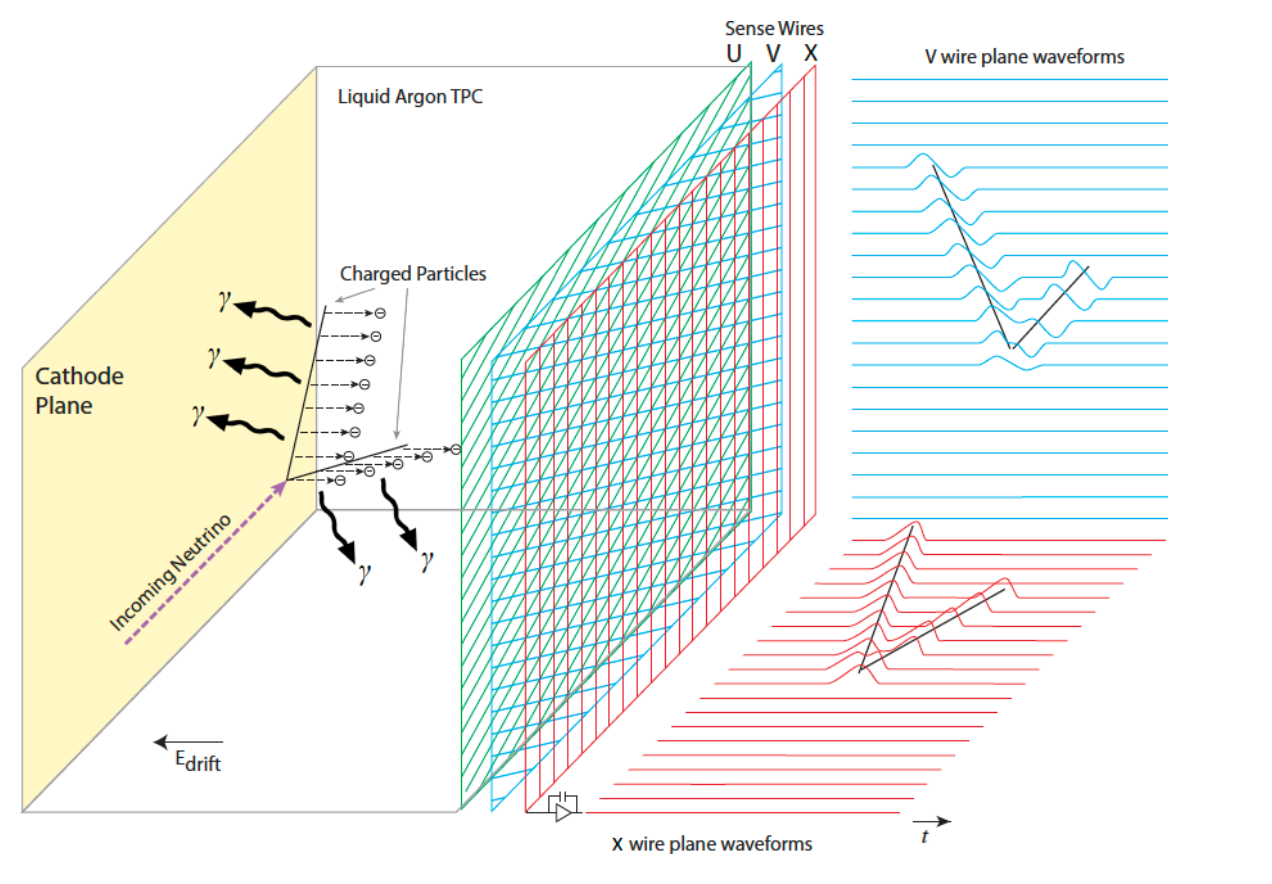
\includegraphics[width=.7\textwidth]{images/LArTPC.png}
		\caption{Sample image, feel free to remove/replace. Source: \href{https://arxiv.org/abs/2002.02967}{\color{blue} Introduction to DUNE. Vol 1}}
		\label{far_detector}
	\end{figure}
\end{frame}


\begin{frame}
	% This is where we discuss the specifics of NuGraph2.py. Need to go in detail about the way that the __init__ function operates (i.e. the encode, planenet, and nexusnet files followed by the decoder selection phase)
	\frametitle{Algorithm Structure}
		The entire algorithm depends largely on three main components
		\begin{enumerate} 
			\item \texttt{train.py}
				\begin{itemize}
					\item This Python file takes as input the model parameters and the \texttt{hdf5} data file to be trained. 
					\item Utilizes PyTorch library
					\item Configures the model based on the input parameters (i.e. batch size, epoch, input/hidden features, etc...)
					\item trains the model using the provided data set.
					\item Calls PyTorch lightning Trainer module to train the model.
					\item It calls the following two files;
				\end{itemize}

			\item \texttt{NuGraph.py}
				\begin{itemize}
					\item This file contains all of the network's architecture.
					\item Contains the key functions \texttt{\_\_init\_\_()}\texttt{forward()}, \texttt{training\_step()}, \texttt{validation\_step()}, etc. which are passed to PyTorch LightningModule and utilized by the training module.
				\end{itemize}

			\item \texttt{H5DataModule.py}
		\end{enumerate}
\end{frame}


\begin{frame}
	% This is where we discuss the specifics of NuGraph2.py. Need to go in detail about the way that the __init__ function operates (i.e. the encode, planenet, and nexusnet files followed by the decoder selection phase)
	\frametitle{NuGraph Architecture}
		The NuGraph neural network architecture consists of three major components
		\begin{enumerate} 
			\item 

			\item 
		\end{enumerate}
\end{frame}



\section{Binary Classification of Decay Events}

\begin{frame}
\frametitle{Sample frame title}
	stuff here
\end{frame}



\section{Model Implementation}

\begin{frame}
\frametitle{Title}
	Stuff here
\end{frame}




\end{document}
